\section{Experimental Results}
After analyzing the results of the implemented models on the training set, we aim to assess the performances yielded on the test set.
Table \ref{tab:gaus_eval} shows the results of the Gaussian classifiers for different applications.

\begin{table}[H]
	\resizebox{.5\textwidth}{!}{
		\begin{tabular}{ p{2.5cm} P{1.5cm} P{1.5cm} p{1.5cm}}	
			\hline
			\hline
			& $\tilde{\pi}=0.1$ & $\tilde{\pi}=0.5$
			& $\tilde{\pi}=0.9$ \\
			\hline
			\multicolumn{3}{c}{\hfill Raw features \hfill} \\
			\hline
			Full-Cov 	  & \boxit{red}{.35in}0.656 & 0.337 & 0.700 \\
			Diag-Cov 	  & 0.731 & 0.367 & 0.867 \\
			Tied Full-Cov & 0.681 & 0.315 & 0.705 \\
			Tied Diag-Cov & 0.737 & 0.368 & 0.930 \\	
			\hline
			\multicolumn{3}{c}{\hfill Gaussianized features \hfill} \\
			\hline
			Full-Cov      & 0.679 & 0.336 & 0.727 \\
			Diag-Cov      & 0.760 & 0.377 & 0.911 \\
			Tied Full-Cov & 0.698 & 0.319 & 0.798 \\
			Tied Diag-Cov & 0.824 & 0.379 & 0.942 \\	
			\hline
			\multicolumn{3}{c}{\hfill Gaussianized features, PCA(m=10) \hfill} \\
			\hline
			Full-Cov      & 0.709 & 0.320 & \boxit{red}{.35in}0.681 \\
			Diag-Cov      & 0.767 & 0.332 & 0.886 \\
			Tied Full-Cov & 0.717 & 0.313 & 0.797 \\
			Tied Diag-Cov & 0.720 & \boxit{red}{.35in}0.310 & 0.804 \\
			\hline
			\multicolumn{3}{c}{\hfill Gaussianized features, PCA(m=9) \hfill} \\
			\hline
			Full-Cov      & 0.737 & 0.326 & 0.705 \\
			Diag-Cov      & 0.787 & 0.338 & 0.790 \\
			Tied Full-Cov & 0.733 & 0.322 & 0.827 \\
			Tied Diag-Cov & 0.745 & 0.317 & 0.839 \\	
			\hline	
		\end{tabular}
	}
	\caption{min DCF for Gaussian models for different values of $\tilde{\pi}$ on the test set.}
	\label{tab:gaus_eval}
\end{table}

The above results prove compatible with those yielded on the training test, especially when applying a k-fold cross validation approach (which is more realiable). On the test set, the tied diagonal-covariance model, which proved less effective in the training phase, yields now the best score. Nevertheless, the full-covariance classifier - which was previously the best performing Gaussian model, keeps producing good results. Applying a 10-components PCA proved again beneficial. 

Table \ref{tab:lr_eval} shows the evaluation results of the Logistic Regression models on the test set.

\noindent
\begin{table}[H]
	\resizebox{.5\textwidth}{!}{
		\begin{tabular}{ p{3.15cm} P{1.5cm} P{1.5cm} P{1.5cm}}
			\hline
			\hline
			& $\tilde{\pi}=0.1$ & $\tilde{\pi}=0.5$
			& $\tilde{\pi}=0.9$ \\
			\hline
			\multicolumn{3}{c}{\hfill Raw features \hfill} \\
			\hline
			Log-Reg ($\lambda=10^{-4}$) & 0.704 & 0.337 & 0.642  \\
			Quad-LR ($\lambda=0$)       & 1.000 & 1.000 & 0.900 \\
			\hline
			\multicolumn{3}{c}{Z-normalized features} \\
			\hline
			Log-Reg($\lambda=10^{-2})$ & 0.682 & 0.331& 0.654 \\
			Quad-LR($\lambda=0$)      & \boxit{red}{.35in}0.638 & \boxit{cyan}{.35in}0.264 & \boxit{red}{.35in}0.533 \\	
			\hline
			\multicolumn{3}{c}{Gaussianized features} \\
			\hline
			Log-Reg($\lambda=0$)       & 0.691 & 0.341 & 0.715 \\
			Quad-LR($\lambda=10^{-2}$) & 0.657 & 0.284 & 0.553 \\	
			\hline
			\multicolumn{3}{c}{Z-normalized features, PCA(m=10)} \\
			\hline
			Log-Reg($\lambda=10^{-2}$) & 0.688 & 0.329 & 0.651  \\
			Quad-LR($\lambda=0$) 	   & 0.670 & \boxit{red}{.35in}0.260 & 0.573  \\	
			\hline
		\end{tabular}
	}
	\caption{min DCF for Logistic Regression models for different values of $\tilde{\pi}$ on the test set.}
	\label{tab:lr_eval}
\end{table}

As already discussed in Chapter 2, quadratic models are expected to outperform linear ones for this specific classification task. The results yielded by the Linear and Quadratic Logistic Regression confirm this statement. 

\noindent
\begin{table}[H]
	\resizebox{.5\textwidth}{!}{
		\begin{tabular}{ p{3.15cm} P{1.5cm} P{1.5cm} P{1.5cm} }
			\hline
			\hline
		& $\tilde{\pi}=0.1$ & $\tilde{\pi}=0.5$
			& $\tilde{\pi}=0.9$ \\
			\hline
			\multicolumn{3}{c}{Raw features} \\
			\hline
			SVC($C=0.1$)              & 1.000 &  0.696 & 0.932\\
			SVC($C=0.1, \pi^{emp}_T$) & 0.964 &  0.575 & 0.927\\
			\hline
			\multicolumn{3}{c}{Z-normalized features} \\
			\hline
			SVC($C=1$)                & 0.670 & 0.318 & 0.664\\
			SVC($C=0.1, \pi^{emp}_T$) & 0.685 & 0.332 & 0.652\\
			\hline
			\multicolumn{3}{c}{Gaussianized features} \\
			\hline
			SVC($C=0.1$)              & 0.705 & \boxit{red}{.3in}0.309 & 0.841\\
			SVC($C=0.1, \pi^{emp}_T$) & 0.695 & 0.323 & 0.787\\		
			\hline
		\end{tabular}
	}
	\caption{min DCF for Support Vector Classifier models, with and without re-balancing, on test set.}
	\label{tab:svc_eval}
\end{table}

As experienced in the training stage, applying a Quadratic LR on Z-normalized features yields the best results. Exploiting a 10-components PCA proved to be of (slight) benefit in this case.

The test scores associated to Support Vector Machine models are report in Table \ref{tab:svc_eval} (linear SVC) and Table \ref{tab:kern_svc_eval} (Kernel SVC). 

\noindent
\begin{table}[H]
	\resizebox{.5\textwidth}{!}{
		\begin{tabular}{ p{5.5cm} P{1.2cm} P{1.2cm} P{1.2cm} }
			\hline
			\hline
			& $\tilde{\pi}=0.1$ & $\tilde{\pi}=0.5$
			& $\tilde{\pi}=0.9$ \\
			\hline
			\multicolumn{3}{c}{Z-normalized features} \\
			\hline
			Poly-SVC($C=0.1$)                          & 0.617 & 0.277 & 0.606 \\
			Poly-SVC($C=0.1, \pi^{emp}_T$)             & 0.650 & 0.278 & 0.572 \\
			RBF-SVC($C=10, log\gamma=-2$)              & 0.705 & \boxit{red}{.3in}0.258 & 0.610 \\
			RBF-SVC($C=10, log\gamma=-2, \pi^{emp}_T$) & 0.752 & 0.260 & 0.516 \\
			\hline
		\end{tabular}
	}
	\caption{min DCF for Kernel Support Vector Classifier models, with and without re-balancing, on test set.}
	\label{tab:kern_svc_eval}
\end{table}

We notice that, differently from the training phase, gaussianization yields better results with linear SVC, for the application of main interest, even though Z-normalization still performs well. On the contrary, it performs poorly on raw data. Balancing the features does not introduce visible advantages. Moreover, as expected, kernel methods perform better than linear SVC with Radial Basis Function Kernel SVC still being the most performing method. Rebalancing is again not detrimental nor beneficial. 

Eventually, Table \ref{tab:gmm_res_eval} shows the results of different GMM models on the test set. We confirm the 8-components full-covariance GMM model as the most effective on Z-normalized features, however on the test set we experience better results on gaussianized features applying a tied-covariance model.
\noindent
\begin{table}[H]
	\resizebox{.5\textwidth}{!}{
		\begin{tabular}{ p{5.4cm} P{1.2cm} P{1.2cm} P{1.2cm}}
			\hline
			\hline
			& $\tilde{\pi}=0.1$ & $\tilde{\pi}=0.5$ & $\tilde{\pi}=0.9$ \\
			\hline
			\multicolumn{2}{c}{Guassianized features} \\
			\hline
			GMM(8 components) 	          & 0.701 & 0.328 & 0.730 \\
			Tied-GMM (16 components)      & 0.742 & \boxit{red}{.35in}0.283 & 0.642 \\
			Diag-GMM (16 components)      & 0.697 & 0.320 & 0.590 \\	
			Tied-Diag-GMM (16 components) & 0.730 & 0.305 & 0.649 \\
			\hline
			\multicolumn{2}{c}{Z-normalized features} \\
			\hline
			GMM (8 components) 	          & 0.785 & \boxit{cyan}{.35in}0.306 & 0.850 \\	
			Tied-GMM (8 components)       & 0.659 & 0.297 & 0.690 \\
			Diag-GMM (16 components)      & 0.781 & 0.328 & 0.711\\
			Tied-Diag-GMM (16 components) & 0.789 & 0.325 & 0.704  \\
			\hline
		\end{tabular}
	}
	\caption{min DCF for Gaussian Mixture Models on test set.}
	\label{tab:gmm_res_eval}
\end{table}


\subsection{Model Fusion}

As done for the training step, we compute the scores in terms of actual DCF using the optimal theoretical threshold and the estimated threshold on the evaluation set. In addition we calibrate the scores using a Linear Logistic Regression Model as described in Section \ref{sec_calib} (with DCF computed on test set). Table \ref{tab:calib_eval} and \ref{tab:calib2_eval} show the the results for the single selected models, whereas \ref{tab:calib_fus_eval} for their fusion. 

\noindent
\begin{table}[H]
	\resizebox{.5\textwidth}{!}{
		\begin{tabular}{ P{4cm} P{2cm} P{3cm} }
			\hline
			\hline
			&  \makecell{$\tilde{\pi} = 0.5$}\\
			\hline	
			& min DCF & act DCF $(t_{opt})$ \\	
			\hline
			RBF SVC  & 0.260 & 0.278 \\
			Quad LR  & 0.264 & 0.280  \\	
			GMM      & 0.306 & 0.340  \\
			\hline
		\end{tabular}
	}
	\caption{minimum and actual DCF for the best performing models}
	\label{tab:calib_eval}
\end{table}

\noindent
\begin{table}[H]
	\resizebox{.5\textwidth}{!}{
		\begin{tabular}{ P{4cm} P{2cm} P{3cm} }
			\hline
			\hline
			&  \makecell{$\tilde{\pi} = 0.5$}\\
			\hline
			& act DCF ($t^*$) & calibrated (LR)	\\	
			\hline
			RBF SVC  &  0.278 & 0.282\\
			Quad LR  &  0.293 & 0.285 \\	
			GMM      &  0.325 & 0.315 \\
			\hline
		\end{tabular}
	}
	\caption{actual estimated and calibrated DCF for the best performing models}
	\label{tab:calib2_eval}
\end{table}

We observe how selecting the optimal threshold is not effective (expect for the GMM model) and that, overall, calibration is beneficial, especially for the Quadratic LogReg and the GMM. 

\noindent
\begin{table}[H]
	\resizebox{.5\textwidth}{!}{
		\begin{tabular}{ P{3.5cm} P{2cm} P{3cm} }
			\hline
			\hline
			&  \makecell{$\tilde{\pi} = 0.5$}\\
			\hline
			& min DCF & act DCF ($t_{opt}$)\\	
			\hline
			SVC + QLR       & 0.252 & 0.261 \\
			SVC + GMM  	    & 0.260 & 0.268 \\	
			SVC + GMM + QLR & \boxit{red}{1.5in}0.247 & 0.258 \\
			\hline
		\end{tabular}
	}
	\caption{minimum and actual DCF for the combination of best performing models}
	\label{tab:calib_fus_eval}
\end{table}

As regards model fusions, we compute the actual DCF using the theoretical threshold and re-use the best values of the norm scaler of the LR model ($\lambda$) during the hyperparameter tuning. We observe how joining models' score proves definitely more effective than using single models and, as already experienced, combining the three best models yields again the best score, both in temrs of min DCF and act DCF, despite obtaining slightly worse results than those yielded on the training set.


\subsection{Different Applications}

In this last section, we assess the performance of our best models for different applications. Figure \ref{fig:roc} shows the ROC curves for the single models and for their fusions. As regards the latter, the curves are almost overlapped, which implies they yield very similar scores, whereas for the former, the RBF SVC and the Quad LogReg perform better than the GMM. 


\begin{figure}[H]
	%\centering
	\subfloat[single models]{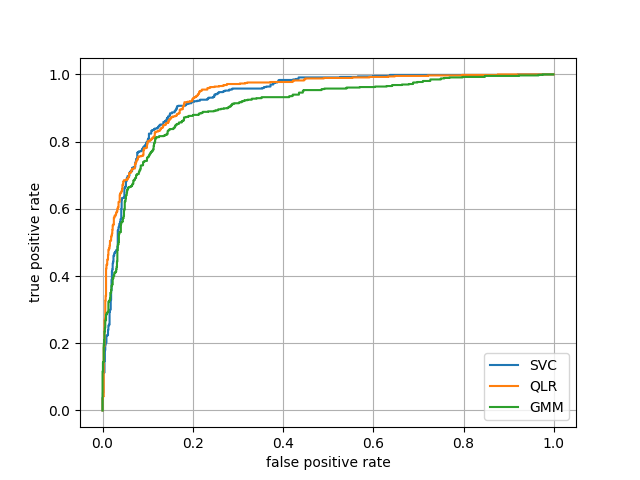
\includegraphics[width=.5\linewidth]{assets/roc_single_models.png}}
	\subfloat[fusion]{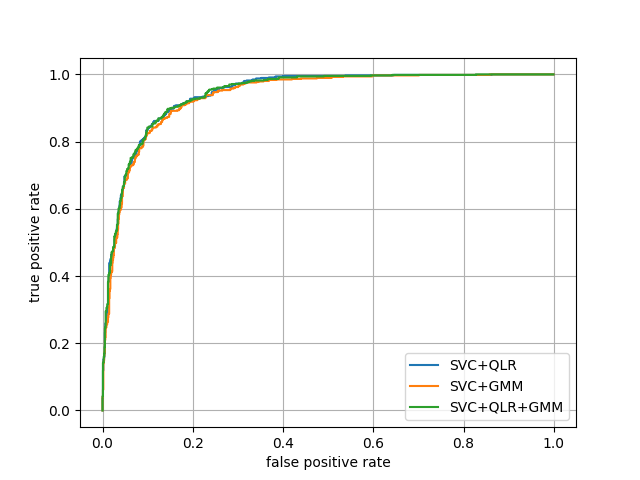
\includegraphics[width=.5\linewidth]{assets/roc_joint_models.png}}
	\caption{ROC plots}
	\label{fig:roc}
\end{figure}


\begin{figure}[H]
	%\centering
	\subfloat[]{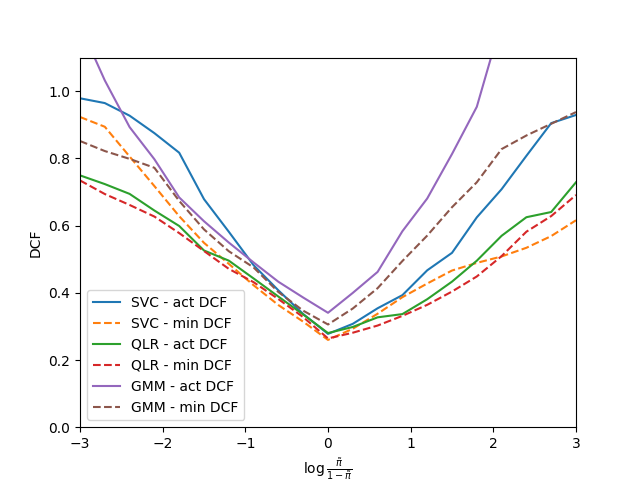
\includegraphics[width=.5\linewidth]{assets/bayes_error.png}}
	\subfloat[]{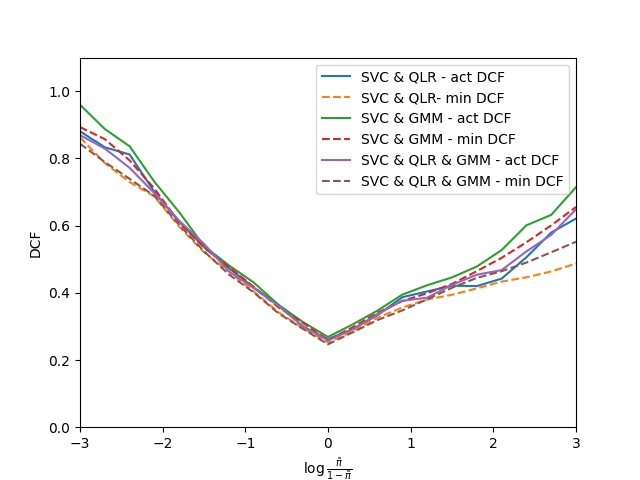
\includegraphics[width=.5\linewidth]{assets/bayes_error_joint.png}}\\
	\subfloat[]{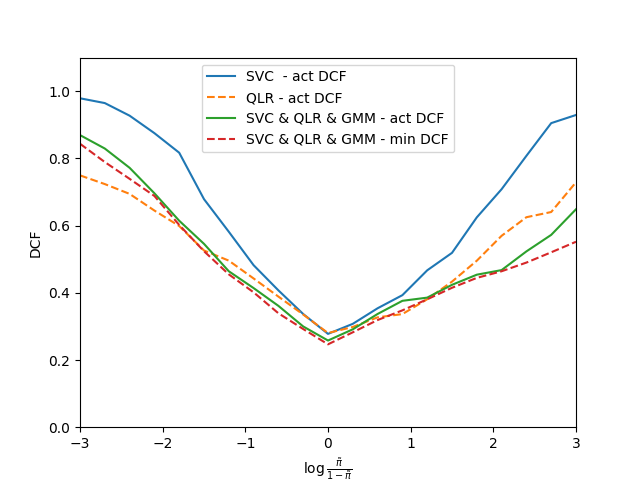
\includegraphics[width=.5\linewidth]{assets/bayes_error_joint2.png}}
	\subfloat[]{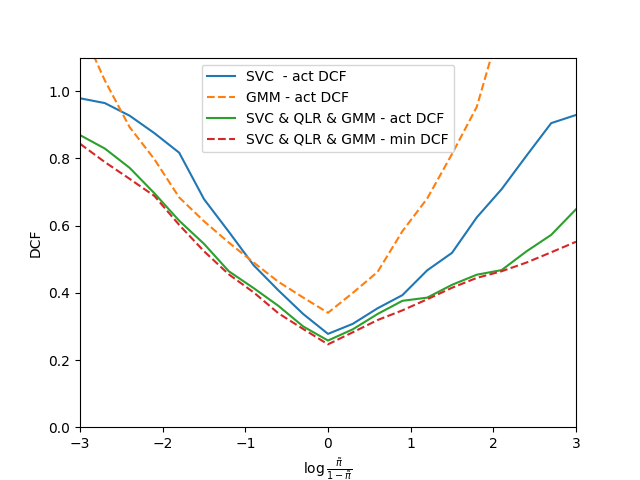
\includegraphics[width=.5\linewidth]{assets/bayes_error_joint3.png}}
	\caption{Bayes error plots against different values of log prior odds}
	\label{fig:bayes_err}
\end{figure}




Figure \ref{fig:bayes_err} shows the mininum and actual DCF against the different applications, i.e. the \columnbreak prior log-odds. We compare single models \textbf{(a)}, fusions \textbf{(b)}, SVC and QLR with fusions \textbf{(c)}, SVC and GMM against fusions \textbf{(d)}.  
Fusions yield similar performances across all the applications and, overall, always outperform single models, with the slight exception of the Quadratic Logistic Regression being better for some applications \textbf{(a, c)}. 

